\subsection{Distributed data management}
\label{ddm}

From the former descriptions, it is evident how LHC data are arguably the most valuable asset of the HEP community.
For this reason, the data are continuously transferred across the grid for several purposes, and a paramount part of the WLCG operations involves Distributed Data Management (DDM) processes.

Indeed, stringent workflows are put in place by the experiments to ensure data distribution and redundancy, thus preventing data loss and guaranteeing reliable accessibility.
For example, the ATLAS experiment has drawn up an accurate plan -- the so-called \textit{computing model} -- describing in detail the data lifecycle \cite{aad2008atlas, calafiura2020design_report, bird2011computing}.
The first data stream happens at the CERN data center, where the raw data acquired by the detectors are applied a combination of electronic and software triggers that filter out uninteresting collisions.
The skimmed data are then archived in the Tier-0 on tape supports for long term storage, and a second copy is sent to one of the Tier-1s through a dedicated network. 
After that, a first-pass reconstruction takes place to retrieve physically meaningful information -- such as particles energy, velocity, scattering angles and so on \sidenote[Luca][notesyellow]{sono giuste queste grandezze?} -- from the electronic signals recorded by the experimental devices.
The derived data are then likewise stored in double copy, one at CERN and one at the same Tier-1 hosting the corresponding raw data.
In this way, two full copies of the same raw and reconstructed data are retained to safeguard data sanity and timely accessibility.
The copy at CERN is archived on durable but slow storage supports, and it serves the purpose of restoring the data in case of losses or corruption. The second copy, instead, is stored on hard drives that are more prone to faults but guarantee a faster reading speed to comply with the repeated data accesses typical of analysis workflows.
Once the data are properly distributed, a second stream takes place at the Tier-1s that provide data-intensive processing facilities for large-scale organized analysis. Here, further (re)processing and calibrations are performed on the reconstructed data, and the derived outputs are stored and shipped on-demand to other sites for subsequent elaborations.
The last part of the data lifecycle is then performed at the Tier-2s, where Monte Carlo data are simulated and sent back to Tier-1s for long term storage. 
Furthermore, the Tier-2s are exploited by smaller groups of researchers to conduct more specialized analyses. In such cases, additional data streams are needed to retrieve the reconstructed data from the Tier-1s and to made the results available to the end-users on their local machines.

% On the other hand, analysis workflows require individual researchers to transfer data of interest for their analyses.
% This potentially requires retrieving data from geographically displaced and heterogeneous storage resources (e.g. tape or disk), transferring them to computing resources that may be situated elsewhere, and transferring the results back to their machines in order to conduct their studies.

As a result, massive amounts of data are constantly moved across the grid%,
% performing two million tasks daily and leveraging over one million computer cores and 1 exabyte of storage
. 
\sidenote[Luca][notesyellow]{introduce FTS} 
In order to achieve that, various services for file transfer have been developed. These are used alternately or concurrently to create a chain of software services that act as interfaces between the end-users and the physical resources.
At the lowest level there is the File Tansfer System (FTS) \cite{karavakis2020fts}, which is configured to reliably interact with diverse storage devices and filesystems, execute fault tolerant transactions and support users authentication.
On top of that, the various collaborations may add other middleware layers as higher level interfaces for the users.
For example, ATLAS uses an open-source framework called Rucio \cite{barisits2019rucio}, that basically orchestrates the transfers, creating a catalog to track data locations, managing replication rules and retries in case of failures and so on.
Clearly, ensuring high service levels is very hard due to the huge volumes transferred, the heterogeneity of the software and hardware components and the large user base.
\sidenote[Luca][notesyellow]{introduce transfer failures}
In practice, occasional faults may happen at various levels and may include a wide range of root causes, provoking failures during the shipment of the files.
These errors may vary from naive ones -- e.g. a mistyped command or the request of a unavailable file -- to more severe software and hardware defects.
For instance, the requesting endpoint or archiving server might be temporarily unreachable (connection shortage).
Likewise, the requested data may be corrupted (checksum error) either due to storage hardware faults or because of unstable connection (network problem).
Also, there might be timeouts when the shipment takes more than the pre-configured waiting window -- e.g. when the desired data are bigger than usual and/or must be retrieved from tape, thus requiring more time.
In addition, errors of different nature may often arise due to the interactions between different middleware layers.
All of these factors, and more, can generate significant service disruptions and infrastructure malfunctions that require prompt intervention.
For this reason, data transfer processes are continuously monitored by teams of shifters. When an issue is detected, the operators report it through the GGUS ticketing system \cite{antoni2008ggus} and experts and site maintainers take care of their solution.
To give an idea of the volumes involved, the ATLAS collaboration alone experienced an average traffic of more than 2 PB per day in 2019 \cite{calafiura2020design_report}, corresponding to roughly 1.5-2 million files moved each day.
Nearly 10\% of these transfers failed producing about 100-200k errors on a daily basis. 
In total, transfer failures generated more than 4k incident reports filed in 2019\footnote{\ggus} for all the LHC experiments (1141 for ATLAS only).
Due to the complexity of the infrastructure and its layered composition, understanding the problem root causes and fixing them demands a great human effort -- more than 100 people were involved in 2019, corresponding to roughly 50 FTEs (Full-Time Equivalent) -- and it may entail undesired disservices.
The average solving time, may vary from a few hours or days -- e.g. in the case of issues that are easy to solve or have already been dealt with in the past -- to entire weeks -- e.g. for unknown problems or more troublesome malfunctions that imply important software or hardware interventions.
In practice, the median solving time for incidents reported by the ATLAS, CMS and LHCb collaborations in 2019 was around 17 days, with a 90\textit{-th} percentile of 44 days and a long right tail extending over 100 days (see \cref{fig:ggus_time}).
\begin{figure}
    \centering
    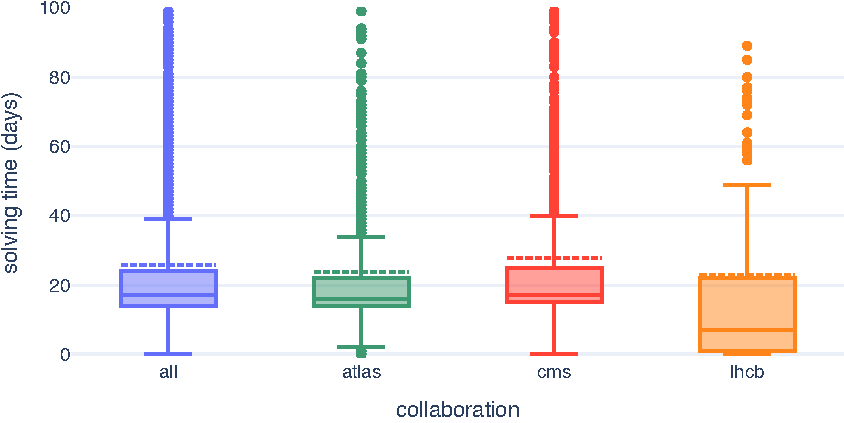
\includegraphics[width=\textwidth]{figures/220_introduction/GGUS_time.pdf}
    \caption{\textbf{Tickets solving time.} Distribution of the solving time for GGUS incidents reported in 2019 by ATLAS, CMS and LHCb collaborations.}
    \label{fig:ggus_time}
\end{figure}
When a transfer failure happens,
% the FTS system produces a log file containing the standard output produced by the transfer process. This information is later parsed and re-organized in a structured format combining the transfers more relevant features and, in particular, an error message composed by the outputs of each subsystem appended one after another.
% Currently, such dataframe is then exposed to the on-duty shifters along with other visualizations for more in depth investigations.
the FTS log files are parsed and the transfers more relevant features are extracted and re-organized in a structured format. 
In particular, this involves collecting the exit status of each of the subsystems responsible for the transfer and appending them to compose a global error message.
This information is then exposed to the on-duty shifters along with other characteristics -- e.g. source and destination endpoints, file size, exchange protocol and so on -- and visualizations -- e.g. time evolution plots or site transfer efficiency -- for more in depth investigations.
% \lc{Here goes some reference to the orders of magnitude at stake, i.e.: 
% \begin{itemize}
%     \item n. tranfers/day (whole or per virtual organization) --> can retrieve from FTS
%     \item ticket/year or month or day (whole or per virtual organization) --> how to retrieve that? is there any official source?
% \end{itemize}
% }

% \lc{Describe current operations and possibly volumes: 
% \begin{itemize}
%     \item Current operations: efficiency matrix + drill down (description + falls)
%     \item average solving time $\rightarrow$ how to retrieve that? is there any official source?
%     \item n. people involved (both shifters and sites) $\rightarrow$ how to retrieve that? is there any official source?
% \end{itemize}
% }
%Current operations are based on a site-centric monitoring approach that involves mainly manual, post-mortem reporting. In this approach, trained operators look at Grafana dashboards that act as a high-level overview of the systems status and try to spot hints of incorrect or undesired behaviours.
Current operations are based on a \textit{site-centric} approach where trained personnel monitors the status of the various services almost 24/7 and tries to spot hints of incorrect or undesired behaviors. In particular, the operators look at Grafana dashboards\footnote{\grafana}
\sidenote[Luca][notesyellow]{Vericare sia possibile condividere snapshot esternamente} to get a high-level overview of the system. A usual starting point is the so-called efficiency matrix (Figure \ref{fig:efficiency_matrix}), where the percentage of successful transfers is reported at customizable levels of granularity -- this may range from global transfers between national cloud infrastructures involving more computing centers to a finer tracking of particular site exchanges or even specific endpoint links. %ranging from cloud to site, endpoint or even space token.
When the efficiency falls below an acceptable threshold, typically 60-70\%, on-duty shifters start to investigate the issue at a lower level by checking \emph{i)} where the error happened, \emph{ii)} how many errors are produced, \emph{iii)} what is the time pattern (temporary, extended or cyclical) and \emph{iv)} which error messages are generated. 
However, this procedure gives rise to many false alarms as it is usual to encounter problems that do not represent a real concern. This typically happens when the failure rate is high just because many transfers were attempted, or there was a transient issue that had already been fixed. 
Also, sometimes unnecessary drill-down activity is performed for actual issues that were already known, as in the case of ongoing tickets or site downtimes, for which reporting is not required.
As a result, many human resources are employed in repetitive tasks of little scientific interest that would enormously benefit from automation. 

\sidenote[Luca][notesyellow]{Describe also why a site-centric approach is not optimal and how a message-centric one could help}
In addition to that, a site-centric strategy as described above has some drawbacks. Firstly, monitoring focuses on spotting where issues occur, while understanding the actual root causes is typically demanded to site experts in a subsequent investigation.
Secondly, problems generating few error messages are usually ignored. This is natural, and to some extent desirable, as having limited resources forces us to address bigger misfunctionings first. However, that could be a potential pitfall in cases where promptly fixing a minor issue may prevent the rising of a more significant and longer to solve defect.

All these problems could be tackled programmatically by standardizing the logging output of all the services. In this way, neat error messages would point directly to the source of the problem, thus allowing complete automation. 
However, the distributed nature of the infrastructure hampers such an approach.
In fact, the opportunistic gathering of computing resources that led to WLCG entails many local configurations that are not easy to address using only a static strategy.
Hence, all these considerations expose the need for an intelligent support tool for speeding up infrastructure management to meet the productivity requirements for the near future.

% Hence, the current approach will no longer meet the productivity requirements in the near future given the limited resources

\subsection{Contribution}
The goal of this work is to discuss a complementary approach to current operations based on an experiment-agnostic, computer-aided strategy to grid monitoring centered on error messages rather than site performances.

In particular, we propose an unsupervised Machine Learning (ML) pipeline to identify clusters of similar failures. These groups of errors retrieved in this way are then exposed to shifters as suggestions of potential issues to investigate further.

\begin{landscape}
\begin{figure}
    \centering
    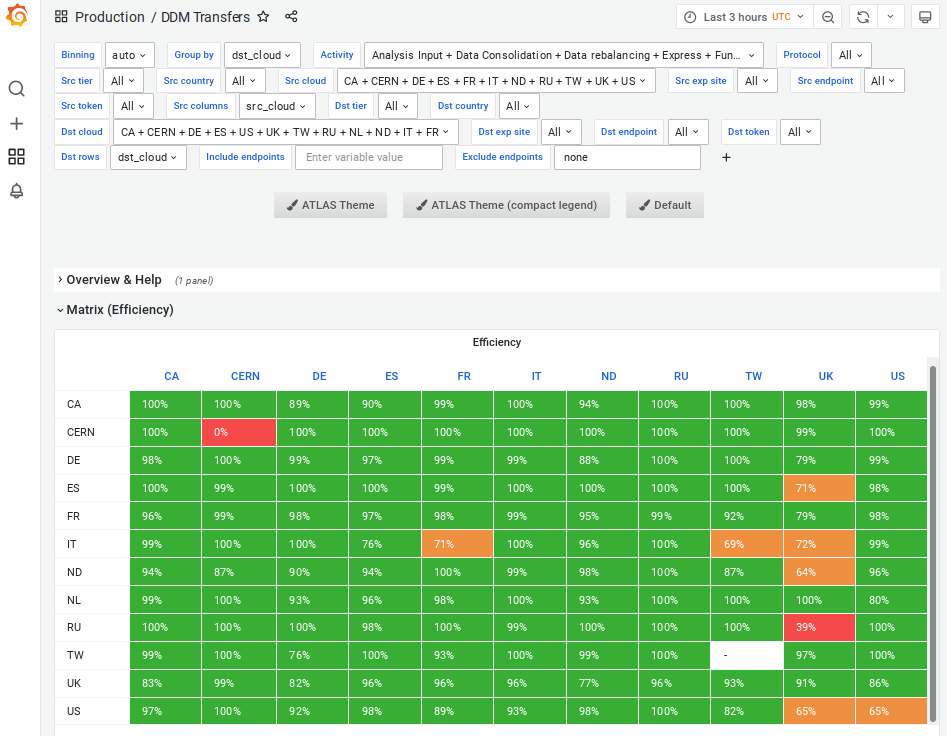
\includegraphics[height=\textwidth]{figures/220_introduction/grafana_efficiency_matrix_narrow1.png}
    \caption{Transfer efficiency matrix from Grafana. Transfer sources are shown as columns and destinations as rows. The drop-down menus at the top allow for custom filtering at the desired level of granularity.}
    \label{fig:efficiency_matrix}
\end{figure}
\end{landscape}
